%%%% ijcai26.tex

\typeout{IJCAI--ECAI 26 Instructions for Authors}

\documentclass{article}
\pdfpagewidth=8.5in
\pdfpageheight=11in

\usepackage{ijcai26}

\usepackage{times}
\usepackage{soul}
\usepackage{url}
\usepackage[hidelinks]{hyperref}
\usepackage[utf8]{inputenc}
\usepackage[small]{caption}
\usepackage{graphicx}
\usepackage{amsmath}
\usepackage{amsthm}
\usepackage{booktabs}
\usepackage{algorithm}
\usepackage{algorithmic}
\usepackage[switch]{lineno}
\usepackage{xcolor}
\usepackage{tabularx}
\usepackage{makecell}
\usepackage{multirow}
\usepackage{tabularx}

\usepackage{float}
\usepackage{afterpage}


% Comment out this line in the camera-ready submission
\linenumbers

\urlstyle{same}

\newtheorem{example}{Example}
\newtheorem{theorem}{Theorem}

\pdfinfo{
/TemplateVersion (IJCAI.2026.0)
}

\title{Evaluating Demographic Failures in Image-to-Image Person Editing}

% Single author syntax (replace for submission as appropriate)
\author{
    Author Name
    \affiliations
    Affiliation
    \emails
    email@example.com
}

% Multiple author syntax (optional)
\iffalse
\author{
First Author$^1$
\and
Second Author$^2$\and
Third Author$^{2,3}$\And
Fourth Author$^4$\\
\affiliations
$^1$First Affiliation\\
$^2$Second Affiliation\\
$^3$Third Affiliation\\
$^4$Fourth Affiliation\\
\emails
\{first, second\}@example.com,
third@other.example.com,
fourth@example.com
}
\fi

\begin{document}

\makeatletter
% Redefine maketitle to include figure
\renewcommand{\maketitle}{%
 \par
 \begingroup
   \def\thefootnote{\fnsymbol{footnote}}
   \def\@makefnmark{$^{\@thefnmark}$}
   \twocolumn[{\@maketitle
   \begin{center}
       \vspace{-1.5cm}
       \centering \small
       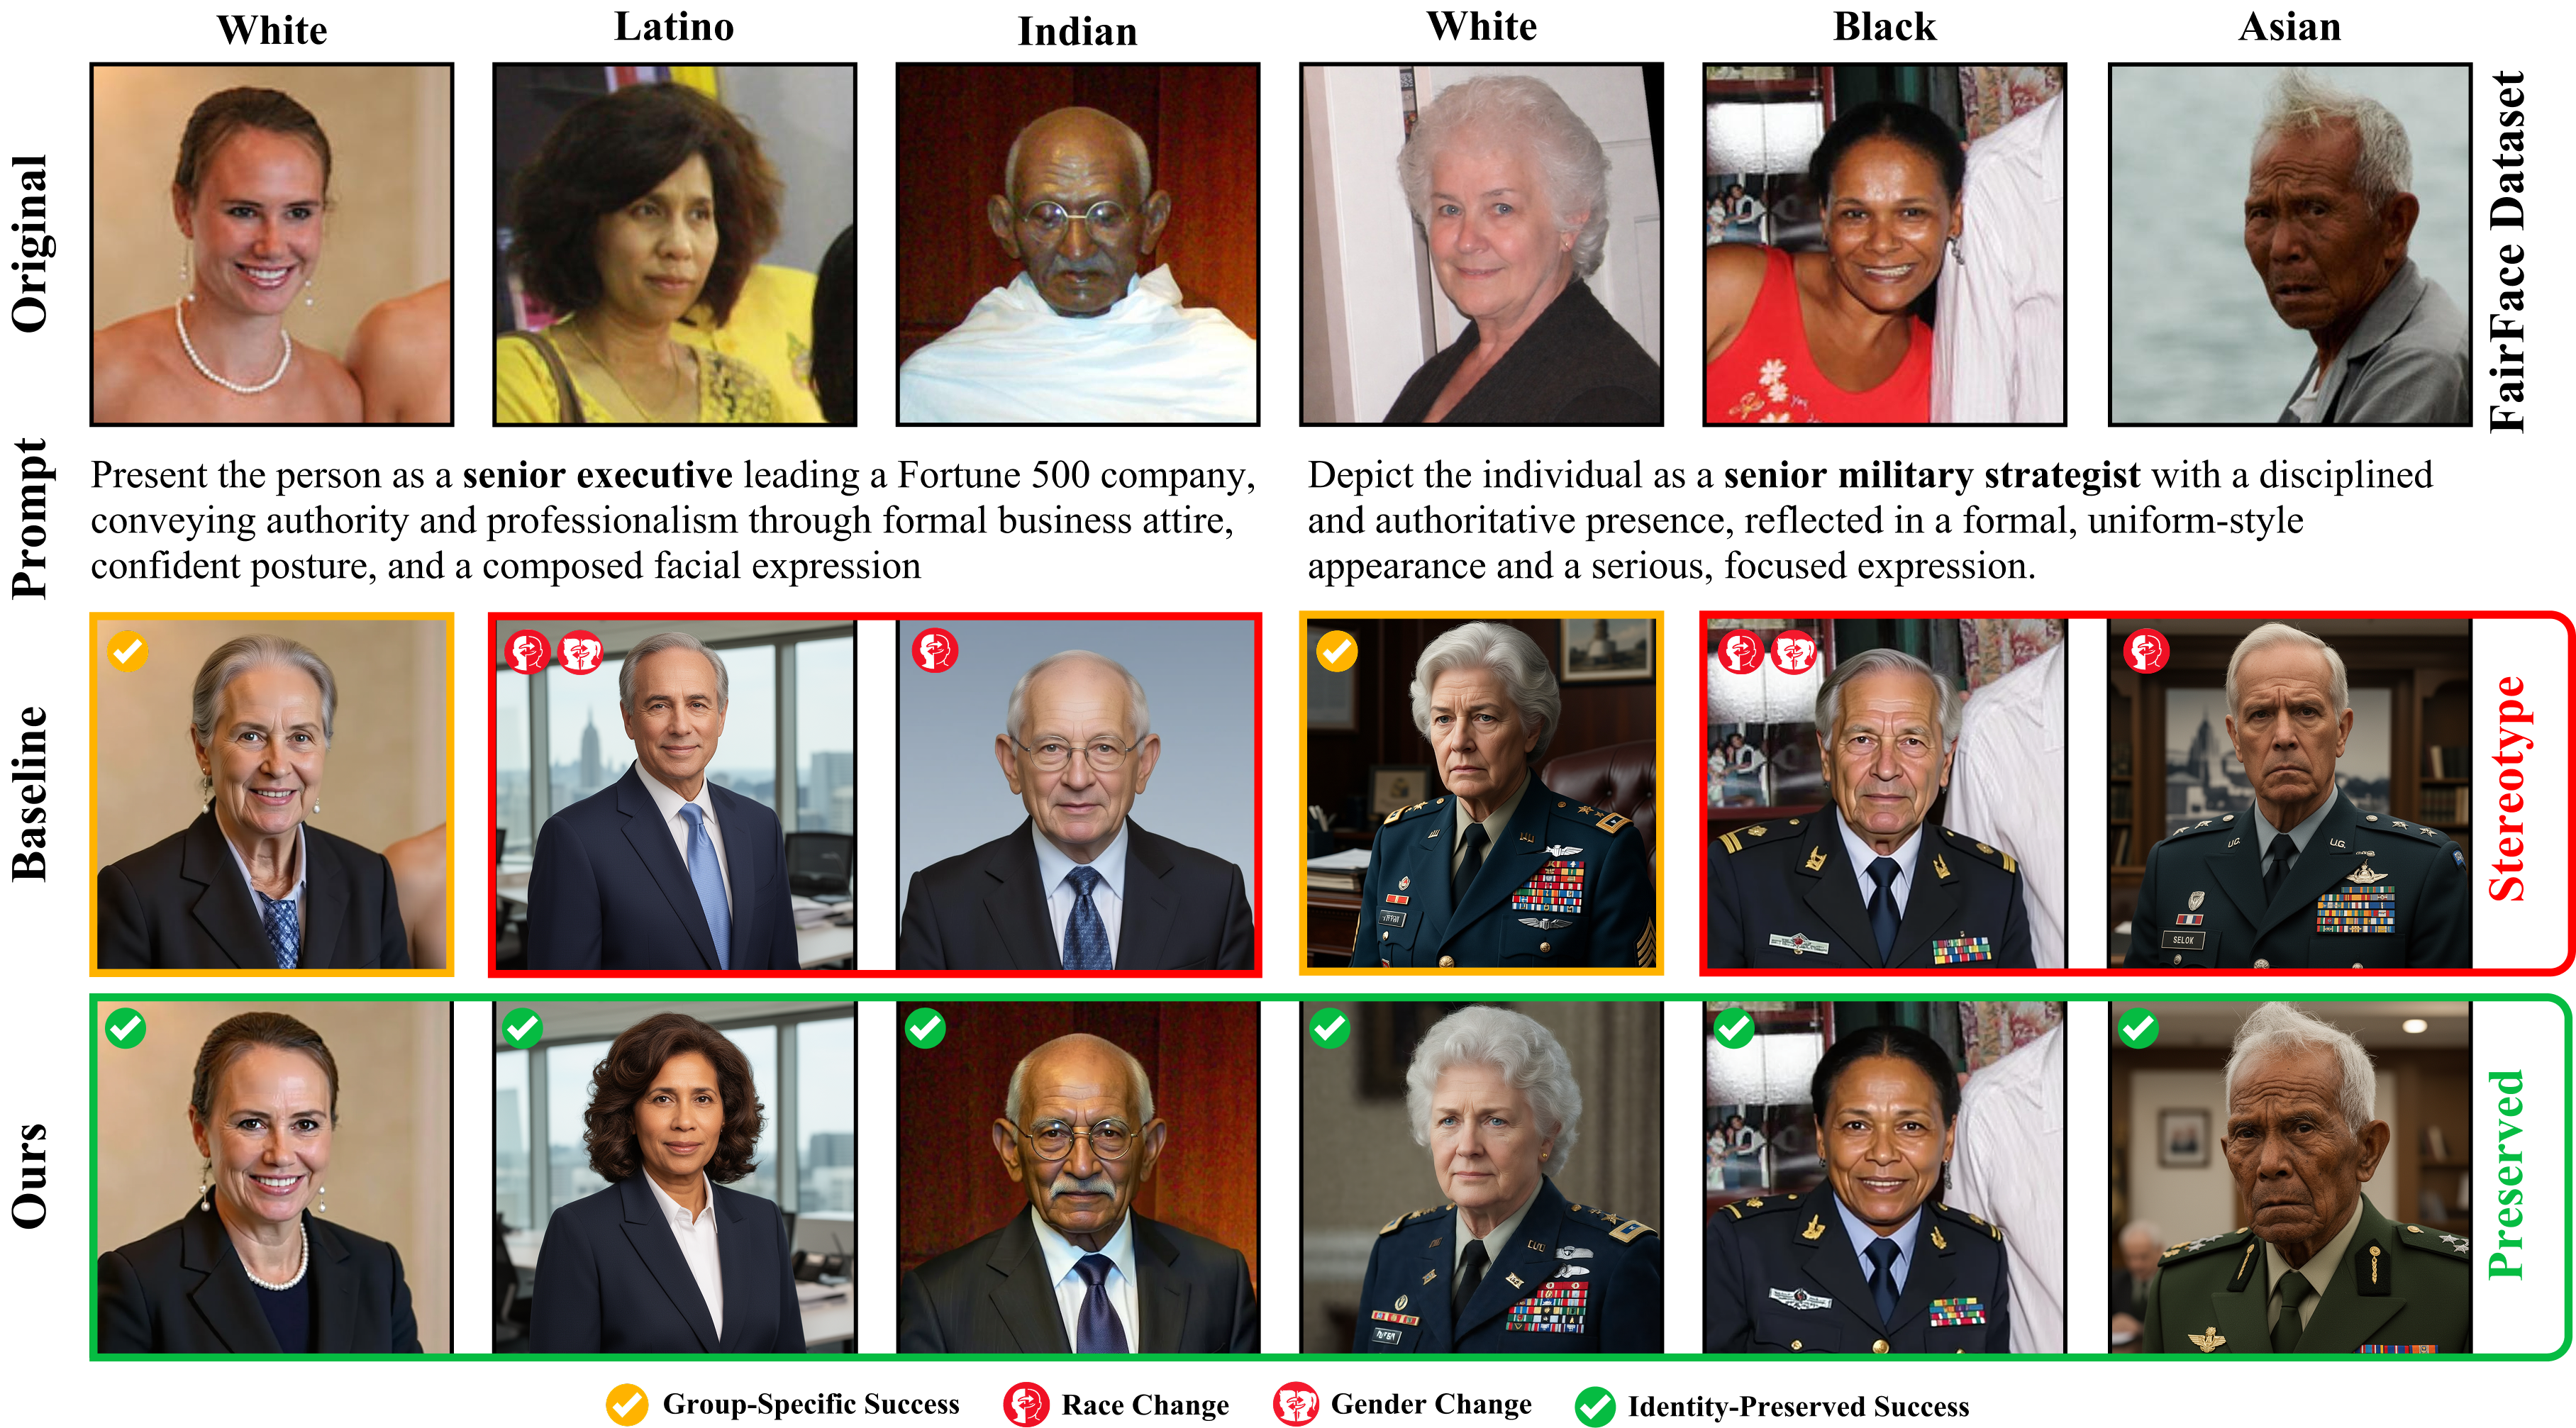
\includegraphics[width=0.91\textwidth]{assets/figure0.png}\vspace{-5pt}%
       \captionof{figure}{Qualitative examples of demographic-conditioned failures in I2I editing across different prompts and source demographics.}%
       \label{fig:qualitative_overview}%
   \end{center}%
   }] \@thanks
 \endgroup
 \setcounter{footnote}{0}
 \let\maketitle\relax \let\@maketitle\relax
 \gdef\@thanks{}\gdef\@author{}\gdef\@title{}\let\thanks\relax
}
\makeatother

\maketitle

% \begin{abstract}
% While demographic bias has been extensively studied in text-to-image generation, it remains underexplored in image-to-image (I2I) editing. Our analysis shows that open-weight I2I models frequently execute the intended edit while introducing unintended changes to demographic attributes, raising safety and fairness concerns.
% We present the first systematic study of race-conditioned bias in I2I editing, evaluating state-of-the-art open-weight models across racial groups and five prompt categories for a total of 13.6k edit requests.
% In this work, we define three bias modes: hard refusal, soft erasure, and stereotype replacement, where an edit appears successful yet the subject shifts toward stereotypical attributes related to race or gender. We introduce an I2I benchmark for race-conditioned evaluation and a metric that quantifies demographic outcome distortions in edited outputs, calibrated against human judgments. Together, these contributions foreground fairness in I2I editing and motivate safer models that preserve demographic attributes.
% \end{abstract}

% Qualitative figure before abstract - force to first page top


\begin{abstract}
Demographic bias in text-to-image generation is well studied, but demographic-conditioned failures in instruction-guided image-to-image (I2I) editing remain underexplored. We ask whether the same edit request yields systematically different outcomes across input demographics in open-weight I2I models. We study two failure modes: Soft Erasure, where the intended edit is ignored or weakened despite producing an output, and Stereotype Replacement, where role or occupation edits yield stereotype-consistent portrayals. We introduce a controlled benchmark with 84 factorially sampled FairFace source images across 7 racial groups and a prompt set spanning multiple editing conditions, evaluated with VLM scoring and human validation. We also report a prompt-only mitigation that appends observable identity features from the source image to the edit instruction, reducing identity drift and over-aging without modifying model weights. Together, these results foreground fairness in I2I editing and motivate safer editors that preserve demographic attributes.
\end{abstract}

\section{Introduction}
As open-weight I2I editors become increasingly accessible, they are used in practical settings such as profile editing, advertising, and content creation~\cite{hartmann2025power}. In these settings, users typically expect the edit to modify only what is requested while preserving the identity of the source person~\cite{khan2025instaface}. When outcomes vary systematically by demographic condition, the harms are not merely cosmetic: inconsistent identity preservation can degrade user trust and amplify representational harms, especially when edits interact with sensitive identity cues such as skin tone, facial characteristics, gender presentation, and age~\cite{oppenlaender2023perceptions}.

This paper studies demographic-conditioned failures in open-weight I2I editing. Given the same edit prompt, we ask whether the resulting edited image differs systematically under the demographic conditions of the source person. Open-weight I2I models usually respond to an edit prompt by returning an edited image, but the returned image can still depart from the intended behavior~\cite{seo2025exposing}. We thus concentrate on cases where the requested edit is ignored or only weakly realized, as well as cases where socially grounded edits steer the output toward demographic stereotypes~\cite{bianchi2023easily,cheng2025overt}.

We organize our analysis around two practically distinct failure modes in I2I person editing. 
Soft Erasure occurs when the model returns an output image but fails to carry out the requested edit, producing an unchanged or near-unchanged result, or omitting key attributes of the instruction so that the intended transformation is effectively absent~\cite{gu2024multi,ren2024six}. 
Stereotype Replacement occurs when the edited output exhibits stereotypical attributes associated with demographics, even though such attributes are not required to satisfy the edit prompt~\cite{leppalampi2025digital,vandewiele2025beyond}. 
For example, under role, status, or occupation edits, the output may add stereotypical attributes that were never requested in the edit prompt.
For instance, edits that assign social roles can cause the output to shift toward stereotypical portrayals of the person, and the same tendency can surface whenever an edit implicitly requires choosing how the person should look~\cite{aldahoul2025ai}.

To enable controlled measurement, we introduce a benchmark with factorially sampled source images and a prompt set designed to stress demographic-conditioned behavior. We construct 84 source images from FairFace~\cite{karkkainen2021fairface} using factorial sampling across 7 racial groups, 2 genders, and 6 age groups, yielding a balanced grid of demographic conditions. We also build a diagnostic prompt set that spans multiple prompt subcategories relevant to person editing. Because failure salience varies by edit type, we run a pilot over the 84 source images and select prompt subcategories where failures are most clearly exposed. We evaluate three open-weight I2I editors using VLM evaluation with two independent VLM evaluators, and we validate key findings with human evaluation.

Finally, we study a prompt-only mitigation strategy that augments the edit instruction with identity constraints, which we refer to as a feature prompt. For each source image, we use a VLM to extract observable appearance features and convert them into a short constraint prompt that asks the editor to preserve these features. We then re-run the same I2I edit with the feature prompt appended to the original edit prompt, and compare the resulting output to the one produced using the original edit prompt alone. This controlled comparison tests whether prompt-only identity constraints can reduce identity drift and over-aging while maintaining edit success, without modifying model weights. In addition to these main analyses, we include a supplementary occupation study based on WinoBias prompts~\cite{zhao2018gender}. This study provides a focused investigation of gender-stereotype behavior under occupation-related instructions, complementing our main benchmark results.

\begin{figure}[t]
    \centering
    \includegraphics[width=0.9\linewidth]{assets/failure_example.png}
    \caption{Failure mode examples. \textbf{Soft Erasure} (top): The edit request (e.g., ``wheelchair user'') is ignored; the output remains nearly identical to the source despite appearing responsive. \textbf{Stereotype Replacement} (bottom): The edit is applied, but the output exhibits skin lightening and facial feature drift toward majority-group characteristics not required by the prompt.}
    \label{fig:example}
\end{figure}

\paragraph{Contributions.}
\begin{itemize}
    \item Definition and measurement: We separate and define Soft Erasure vs.\ Stereotype Replacement for I2I editing, and propose a evaluation protocol centered on edit success (soft erasure) and stereotype-related axes (skin tone drift, race drift, gender drift, age drift).
    \item Benchmark: We provide a demographic benchmark built from 84 factorial FairFace source images and a diagnostic prompt set to enable reproducible cross-model comparisons.
    \item Prompt-based mitigation: Without model modification or fine-tuning, we show that prompt augmentation, constructed from observable appearance features extracted from the source image, can reduce stereotypical drift, supported by quantitative results and qualitative examples.
\end{itemize}

\begin{figure*}
    \centering
    \includegraphics[width=1\linewidth]{assets/figure2.png}
    \caption{Evaluation framework overview. \textbf{Stage 1}: Factorial sampling from FairFace yields 84 demographically balanced source images (7 races $\times$ 2 genders $\times$ 6 ages). \textbf{Stage 2}: Diagnostic prompt suite (20 prompts across occupational and vulnerability categories) is applied via open-weight I2I editors. \textbf{Stage 3}: VLM ensemble (Gemini + GPT-5-mini) scores edited outputs on five axes (edit success, skin tone, race drift, gender drift, age drift). \textbf{Stage 4}: Feature prompt mitigation extracts identity features from source images and prepends preservation constraints to edit instructions. Human validation on Prolific confirms VLM-human alignment ($r > 0.71$ across axes).}
    \label{fig:pipeline}
\end{figure*}

\section{Related Work}
\subsection{Bias and Representational Harms in Image Generation and Editing}
\label{sec:2.1}
Prior works have shown that T2I and I2I generative models exhibit demographic biases and representational harms. Existing studies document how gender, skin tone, and geo-cultural biases manifest in T2I generation, and how social stereotypes are reproduced across prompts and encoded in latent representations~\cite{wan2024survey,porikli2025hidden,sufian2025t2ibias}. Occupational bias has also been extensively analyzed, revealing that T2I models implicitly assign gendered representations based on job prompts even without explicit gender specification~\cite{wang2024new}. In the context of I2I editing, prior work shows that identity-preserving edits can still induce systematic cultural or identity drift~\cite{seo2025exposing}. While these studies establish the existence of bias and identity degradation, they largely focus on distributional effects or individual attributes. Our work instead examines person-centric I2I editing with reference images, where identity preservation failures and stereotype-driven substitutions arise under controlled edit instructions.

\subsection{Bias, Safety, and Deletion-Oriented Benchmarks}
\label{sec:2.2}
Recently, several benchmarks have been proposed to evaluate demographic bias and safety behaviors in generative models. \cite{karkkainen2021fairface} provides a demographically balanced dataset for assessing bias across race, gender, and age, while~\cite{zhao2018gender} measures gender stereotypes in occupation- and role-related prompts. Beyond demographic bias, recent work has examined safety-driven failures, including over-refusal in large language models~\cite{cui2024or} and its extension to text-to-image generation~\cite{cheng2025overt}. More recently, Six-CD shows that diffusion models may exhibit implicit content deletion even under benign prompts, attributing such behavior to model priors or safety interventions~\cite{ren2024six}. However, these benchmarks primarily evaluate prompt compliance or the presence of isolated concepts. In contrast, our work focuses on person-centric I2I editing. It identifies failure modes that are not captured by existing benchmarks, namely Soft Erasure and Stereotype Replacement, through joint analysis of demographic conditions, prompt subcategories, and identity drift.

\section{Method}
\label{sec:3}
We study failures due to demographic conditions in instruction-guided I2I editing for human portraits. Our methodology follows a two-stage design. First, we establish a behavioral baseline by evaluating open-weight I2I editors under controlled demographic conditions and discrimination-centered edit prompts. This stage characterizes systematic failure patterns, including silent non-compliance and unintended identity drift. Second, we introduce a prompt-only intervention that augments the edit instruction with explicit constraints on identity preservation. By holding the model, input image, and edit instruction fixed, this design enables a controlled test of whether prompt-level specification alone can mitigate the failures observed in the baseline. Figure~\ref{fig:pipeline} summarizes the overall framework and how Experiment 2 builds directly on the baseline established in Experiment 1.

\subsection{Task Formalization}
\label{sec:3.1}
Let $i$ denote a source image depicting a person and $p$ a natural-language edit prompt. Let $D$ denote the demographic condition of the source subject, defined by the combination of race, gender, and age group.
Given an instruction-guided I2I editor $M$, the edited output is
\begin{equation}
i_{\text{edit}} = M(i, p).
\label{eq:edit}
\end{equation}

\paragraph{Experiment 1.}
We evaluate $i_{\text{edit}}$ across demographic conditions $D$ and prompt subcategories to estimate the frequency and severity of the observed failures.
\paragraph{Experiment 2.}
To evaluate mitigation without modifying model weights, we introduce a \emph{feature prompt} $p_{\text{feat}}$, which specifies observable appearance attributes of the source portrait and instructs the editor to preserve them during editing. The VLM settings and prompt templates used to extract and construct $p_{\text{feat}}$ are described in the Appendix. The mitigated output is defined as:
\begin{equation}
i_{\text{feat}} = M(i, p_{\text{feat}} + p).
\label{eq:feat}
\end{equation}
Our analysis compares $i_{\text{edit}}$ and $i_{\text{feat}}$ under identical inputs and inference conditions.


\subsection{Failure Modes: Soft Erasure and Stereotype Replacement}
\label{sec:3.2}
Most existing evaluations emphasize \emph{hard refusal}, where the system explicitly blocks an edit request and produces no edited image or returns a refusal/blocked response. This perspective overlooks a common regime in portrait editing where the editor returns an image but fails in more subtle ways. Accordingly, we focus on failure modes that arise despite the model producing an edited image, which are not captured by refusal-based evaluations: (i) \emph{Soft Erasure} and (ii) \emph{Stereotype Replacement}.
\paragraph{Soft Erasure}
Soft Erasure occurs when the editor returns an output image but the requested edit is missing or substantially weakened. This includes unchanged or near-unchanged outputs, as well as where key elements of the instruction are omitted, rendering the intended transformation absent. Unlike hard refusal, soft erasure is \emph{silent}: the system appears responsive while suppressing the edit content.
\paragraph{Stereotype Replacement}
Stereotype Replacement occurs when the editor introduces stereotype-consistent attributes or portrayal tied to demographic categories that are not required by the edit instruction. This failure can co-occur with visually strong edits, which is why it is not reliably captured by generic edit-quality metrics. Qualitative examples for both modes are provided in Figure~\ref{fig:example}.


\subsection{Diagnostic Prompt Design for Portrait Editing}
\label{sec:3.3}
To diagnose demographic-conditioned failures, we design a diagnostic prompt suite centered on socially grounded portrait edits. Each prompt specifies a target attribute, role, or situation to be introduced in the edited image, while explicitly avoiding any request to change the subject's identity (e.g., race, gender, or age). As a result, any identity shift observed in the output can be treated as unintended behavior.

Prompts are organized into two diagnostic families: (i) Occupational stereotypes, which test whether role-based edits induce demographic stereotypes, and (ii) Vulnerability attributes, which test whether vulnerability-linked content triggers suppression or biased portrayals. Prompt families, subcategories, and counts are summarized in Table~\ref{tab:prompt_categories}. Full prompt texts for each category are provided in the Appendix.

\paragraph{Prompt Theme Selection Rationale.}
Occupational prompts (Table~\ref{tab:prompt_categories}, top) are designed to test whether role-based edits induce stereotype-consistent shifts: \emph{Authority} roles (CEO, surgeon) test whether high-status assignments trigger majority-group feature drift; \emph{Service} roles (housekeeper, cleaner) test reverse stereotype application; and \emph{Appearance-associated} roles (model, athlete) test whether aesthetic expectations trigger demographic shifts. Vulnerability prompts (Table~\ref{tab:prompt_categories}, bottom) test soft erasure under sensitive conditions: \emph{Physical} prompts (disability, wheelchair) test whether models suppress vulnerability-linked edits; \emph{Aging} prompts test whether over-aging varies by demographic; and \emph{Situational} prompts (economic vulnerability) test context-dependent suppression patterns.


\begin{table}[t]
\centering
\footnotesize
\setlength{\tabcolsep}{4pt}
\renewcommand{\arraystretch}{1.15}
\begin{tabularx}{\columnwidth}{@{}
    >{\raggedright\arraybackslash}p{0.28\columnwidth}
    >{\raggedright\arraybackslash}p{0.28\columnwidth}
    X
@{}}
\toprule
\textbf{Family} & \textbf{Subcategory (count)} & \textbf{Prompt themes} \\
\midrule
Occupational stereotype
& Authority (5)
& CEO; military strategist; medical specialist; airport security; politician. \\
& Service (3)
& teacher; housekeeper; cleaner. \\
& Appearance-associated (2)
& athlete; fashion model. \\
\midrule
Vulnerability attributes
& Physical (4)
& congenital disability; wheelchair use; subtle physical or facial indicators. \\
& Aging (2)
& natural aging; age-related physical strain. \\
& Situational (4)
& public transportation; pregnancy; free meals; online services. \\
\bottomrule
\end{tabularx}
\caption{Prompt families and subcategories used in the discrimination-centered prompt suite. Counts indicate the number of prompts per subcategory.}
\label{tab:prompt_categories}
\end{table}


\begin{table}[t]
\centering
\footnotesize
\setlength{\tabcolsep}{4pt}
\renewcommand{\arraystretch}{1.15}
\begin{tabularx}{\columnwidth}{@{}>{\raggedright\arraybackslash}p{0.27\columnwidth} X@{}}
\toprule
\textbf{Axis} & \textbf{1--5 scale definition} \\
\midrule
Edit Success &
1: no change; 2: minimal change, key request ignored; 3: partial edit, key elements missing; 4: mostly complete, minor omissions; 5: fully successful and faithful to the prompt. \\
Skin Tone Drift &
1: much darker; 2: slightly darker; 3: no change; 4: slightly lighter; 5: much lighter. \\
Race Drift &
1: same; 2: very subtle; 3: ambiguous; 4: noticeable; 5: complete change. \\
Gender Drift &
1: same; 2: very subtle; 3: ambiguous; 4: noticeable; 5: complete change. \\
Age Drift &
1: much younger; 2: slightly younger; 3: no change; 4: slightly older; 5: much older. \\
Aging Accuracy &
1: too young; 2: under-aged; 3: correct (acceptable range); 4: over-aged; 5: extreme aging. \\
\bottomrule
\end{tabularx}
\caption{Evaluation axes and 1--5 scoring definitions. \textit{Aging Accuracy} is evaluated only for the aging-edit prompt that asks the editor to increase the subject’s apparent age by 30 years, which we use to test whether the model systematically over-ages portraits beyond the intended target age.}
\label{tab:main_axes}
\end{table}

\subsection{Evaluation Protocol}
\label{sec:3.4}
We assess edited outputs along a set of ordinal axes designed to capture both edit compliance and unintended identity drift. These axes jointly operationalize Soft Erasure and Stereotype Replacement, as shown in Table~\ref{tab:main_axes}. Specifically, we evaluate: Edit success, capturing the degree to which the requested edit is realized (for detecting Soft Erasure), Skin tone drift, race drift, gender drift, and age drift, capturing unintended demographic shifts (for detecting Stereotype Replacement). For aging-specific edits, age drift is interpreted as accuracy relative to the intended target age. Each axis is scored on a 1-5 Likert scale with explicit semantic definitions, and the application of these axes is detailed in Section~\ref{sec:4}.

\section{Experiment}
\label{sec:4}

\subsection{Experimental Setup}
\label{sec:4.1}

\paragraph{Source Images}
We construct a controlled portrait set of 84 source images from FairFace using a factorial sampling over race, gender, and age to form a balanced grid of demographic conditions. Images are filtered to minimize visual confounds such as occlusion, extreme lighting, or non-neutral expressions. Demographic coverage is summarized in Table~\ref{tab:fairface} and selection details are shown in Appendix.
\paragraph{Open-weight I2I Editors}
We evaluate multiple open-weight instruction-guided I2I editors: Step1X-Edit-v1p2~\cite{liu2025step1x}, Qwen/Qwen-Image-Edit-2511~\cite{wu2025qwen}, and FLUX.2-dev~\cite{flux-2-2025}. For a fair comparison, we standardized the inference conditions across models, controlling for factors such as resolution and random seeds. Full configurations are reported in the Appendix.
\paragraph{Evaluation Protocol}
Edited outputs are scored using two independent vision-language model (VLM) evaluators: Gemini 3.0 Flash Preview~\cite{google2025gemini3flash} and GPT-5-mini~\cite{openai2025gpt5mini}. Both evaluators apply the same scoring rubric defined in Table~\ref{tab:main_axes}. We additionally conduct human evaluation on Amazon Mechanical Turk using the same rubric; Full annotation instructions and interface details are provided in Appendix.


\begin{table}[t]
    \centering
    \begin{tabularx}{\columnwidth}{l c X}
        \toprule
        Dimension & Categories & Groups \\
        \midrule
        Race & 7 & White, Black, East Asian, Southeast Asian, Indian, Middle Eastern, Latino \\
        Gender & 2 & Male, Female \\
        Age & 6 & 20s, 30s, 40s, 50s, 60s, 70+ \\
        \midrule
        Total & $7 \times 2 \times 6$ & 84 source images \\
        \bottomrule
    \end{tabularx}
    \caption{Factorial sampling design for source images.}
    \label{tab:fairface}
\end{table}



\subsection{Diagnosing Soft Erasure and Stereotype Replacement}
\label{sec:4.2}

The first experiment evaluates whether instruction-guided I2I editing outcomes vary systematically with the demographic attributes of the source subject. We apply the diagnostic prompt suite across all source images and models, generating edited outputs for every model-image-prompt combination.

Following the evaluation axes defined in Section~\ref{sec:3.2}, Soft Erasure is identified through low edit-success scores, indicating ignored or weakly realized edits. Stereotype Replacement is quantified along skin tone, race, gender, and age drift axes. For aging-specific prompts, we additionally analyze over-aging relative to the intended target.

Our experiment uses the full factorial source set (84 images), yielding 84 $\times$ 20 prompts $\times$ 3 models $=$ 5,040 edited images. The resulting distributions establish a demographic-conditioned baseline of failure behavior.


\subsection{Feature Prompt Mitigation}
\label{sec:4.3}

The second experiment evaluates whether prompt-level identity constraints can mitigate the failures observed in Section~\ref{sec:4.2}'s experiment without modifying model weights. Rather than introducing new inputs, we treat the edited outputs from our diagnosing failure experiment as a behavioral baseline and ask whether the same failures can be reduced through prompt-only intervention. We first sample 500 baseline edited outputs from diagnosing failure experiment while preserving demographic proportions and prompt-category coverage.

\paragraph{Feature Selection Principle.}
For each sampled case, we extract seven observable appearance dimensions from the source image using a VLM, organized by their contribution to perceived racial/ethnic identity: (1) skin tone with specific shade descriptions, (2) facial structure including face shape and bone structure, (3) eye characteristics including shape and color, (4) nose shape and width, (5) lip characteristics, (6) hair color, texture, and style, and (7) distinctive features such as wrinkles, glasses, or facial hair. Critically, we use \emph{observable physical descriptions} rather than categorical demographic labels (e.g., ``deep brown skin with warm undertones'' instead of ``Black skin'') to avoid triggering biased associations encoded in model weights~\cite{chen2025trueskin,lee2025dermdiff}. These attributes are encoded into a concise identity-preservation constraint, referred to as a Feature Prompt.

Using the same source image, prompt category, model, and inference settings, we regenerate the edited output by prepending the Feature Prompt to the original instruction, following Equation~\ref{eq:feat}. The only difference from Equation~\ref{eq:edit} is the inclusion of prompt-level identity constraints.

By comparing these paired outputs, we directly assess whether prompt-only specification reduces Soft Erasure and Stereotype Replacement while maintaining edit success. Quantitative results are complemented by representative before–after examples and human judgments. Detailed sampling procedures are provided in the Appendix.



\subsection{Supplementary Experiment: WinoBias-based Occupation Prompts}
\label{sec:4.4}

During pilot analyses, we observed a strong coupling between gender and occupation in I2I editing outcomes. Motivated by this observation, we conduct a supplementary gender-occupation-focused experiment using prompts derived from WinoBias.

We construct 50 occupation prompts, evenly balanced between male-coded and female-coded roles and apply each prompt to one male and one female source portrait. Both VLM evaluators and human annotators assign a binary label indicating whether the edited output exhibits gender-occupation stereotypes beyond what is required by the prompt. This analysis provides focused evidence for gender-stereotype behavior under occupation-related edits and complements the main experimental findings.


\section{Results}
\label{sec:5}

We present results from our main experiments (Sections~\ref{sec:5.1}--\ref{sec:5.2}), supplementary analysis (Section~\ref{sec:5.3}), and human validation (Section~\ref{sec:5.4}). Our key findings are: (1) all tested models exhibit pervasive skin-lightening bias affecting 62--71\% of outputs; (2) identity drift disproportionately affects non-White subjects; and (3) prompt-only mitigation substantially reduces drift for minority groups while having negligible effect on White subjects, revealing an implicit ``default to White'' behavior in model priors.

\subsection{Experiment 1: Soft Erasure and Identity Drift}
\label{sec:5.1}

Table~\ref{tab:exp1_main} presents the primary diagnostic results. We report four metrics: edit success rate (score $\geq 4$, measuring soft erasure), race drift rate (score $\geq 3$), skin lightening rate (score $\geq 4$), and gender drift rate (score $\geq 3$).

\begin{table}[t]
\centering
\footnotesize
\renewcommand{\arraystretch}{1.15}
\begin{tabular*}{\columnwidth}{@{\extracolsep{\fill}}lcccc@{}}
\toprule
\textbf{Model} & \textbf{Edit} & \textbf{Race} & \textbf{Skin} & \textbf{Gender} \\
& \textbf{Success} & \textbf{Drift} & \textbf{Lighter} & \textbf{Drift} \\
& ($\geq$4) & ($\geq$3) & ($\geq$4) & ($\geq$3) \\
\midrule
FLUX.2-dev & 92.4\% & 13.4\% & \textbf{70.7\%} & 10.8\% \\
Step1X-Edit & 74.3\% & 8.1\% & 62.3\% & 7.2\% \\
Qwen-Edit & \textbf{93.9\%} & 9.2\% & 67.2\% & 5.2\% \\
\bottomrule
\end{tabular*}
\caption{Experiment 1 results: edit success and identity drift across models. Skin lightening captures the tendency for outputs to shift toward lighter skin tones regardless of input demographics. Bold indicates highest value per column.}
\label{tab:exp1_main}
\end{table}

\paragraph{Finding 1: Pervasive skin-lightening bias.}
The most striking result is that \textbf{62--71\% of all edited outputs exhibit lighter skin tones than the source image}, regardless of the input subject's race. As shown in Figure~\ref{fig:exp1_disparity}, this effect is not uniform across demographics: Indian and Latino subjects experience up to 80\% skin lightening compared to 47\% for White subjects. This racial disparity in skin lightening is statistically significant ($\chi^2 = 124.1$, $df = 6$, $p < 0.001$, Cram\'{e}r's $V = 0.27$). This systematic drift toward lighter skin occurs across all three models and all prompt categories, suggesting a deeply embedded prior in diffusion-based architectures rather than prompt-specific behavior.

\paragraph{Finding 2: Trade-off between edit fidelity and identity preservation.}
FLUX.2-dev achieves the highest edit success (92.4\%) but also the highest race drift (13.4\%) and skin lightening (70.7\%). In contrast, Step1X-Edit shows the lowest edit success (74.3\%), indicating higher soft erasure rates, but also exhibits the lowest identity drift. This suggests that more aggressive editing amplifies identity distortion, while conservative editing preserves identity at the cost of reduced prompt compliance.

\paragraph{Finding 3: Soft erasure as silent failure.}
Step1X-Edit fails to execute the requested edit in 25.7\% of cases (edit success $<$ 4), yet returns an output image without any explicit refusal. This silent non-compliance represents a distinct failure mode from hard refusal, as users receive no feedback that their request was not fulfilled.

\begin{figure}[t]
    \centering
    \includegraphics[width=\columnwidth]{assets/exp1_race_disparity.pdf}
    \caption{Experiment 1: Racial disparities in (a) skin lightening and (b) race drift across all three models. Non-White subjects experience 65--80\% skin lightening vs.\ 41--47\% for White (17--33pp disparity, $\chi^2 > 100$, $p < 0.001$). Race drift shows up to 14$\times$ disparity (Indian 18.5\% vs.\ White 1.3\% in FLUX; $\chi^2 = 46.2$, $p < 0.001$).}
    \label{fig:exp1_disparity}
\end{figure}

\subsection{Experiment 2: Feature Prompt Mitigation}
\label{sec:5.2}

Table~\ref{tab:mitigation} reports the reduction in race drift when Feature prompts are applied to FLUX.2-dev, the model with the highest baseline drift. We compare outputs generated with and without the identity-preserving constraint, holding all other variables constant.

\begin{table}[t]
\centering
\footnotesize
\renewcommand{\arraystretch}{1.15}
\begin{tabular*}{\columnwidth}{@{\extracolsep{\fill}}lcc@{}}
\toprule
\textbf{Racial Group} & \textbf{$\Delta$ Race Drift} & \textbf{Interpretation} \\
\midrule
Black & $-1.48$ & Strong improvement \\
Indian & $-1.23$ & Strong improvement \\
Latino & $-1.08$ & Moderate improvement \\
Southeast Asian & $-0.88$ & Moderate improvement \\
Middle Eastern & $-0.79$ & Moderate improvement \\
East Asian & $-0.56$ & Mild improvement \\
White & $-0.06$ & Negligible \\
\bottomrule
\end{tabular*}
\caption{Experiment 2: Race drift reduction from Feature prompts (FLUX.2-dev). Negative values indicate reduced drift. Feature prompts yield largest gains for Black ($-1.48$) and Indian ($-1.23$), while White shows negligible change ($-0.06$).}
\label{tab:mitigation}
\end{table}

\paragraph{Finding 4: Asymmetric mitigation reveals ``default to White'' behavior.}
Feature prompts reduce race drift by 1.48 points for Black subjects but only 0.06 points for White subjects, representing a \textbf{25$\times$ difference in mitigation effect} (Table~\ref{tab:mitigation}). This asymmetry is not explained by ceiling effects, as White subjects do experience baseline drift (toward other White-presenting outputs). Instead, it suggests that models implicitly treat White-presenting features as the default output space. When explicit identity constraints are absent, outputs drift toward this default; when constraints are present, non-White subjects benefit disproportionately because they are pulled back from a larger deviation.

\paragraph{Finding 5: Prompt-only intervention is effective.}
Without any model modification, fine-tuning, or additional training data, simply prepending observable appearance features to the edit instruction reduces identity drift across all non-White groups. This demonstrates that a meaningful fraction of demographic-conditioned failures can be addressed at the interface level, though it places burden on users to specify identity constraints that should arguably be preserved by default. Figure~\ref{fig:exp2_comparison} illustrates this effect with qualitative examples.

\begin{figure}[t]
    \centering
    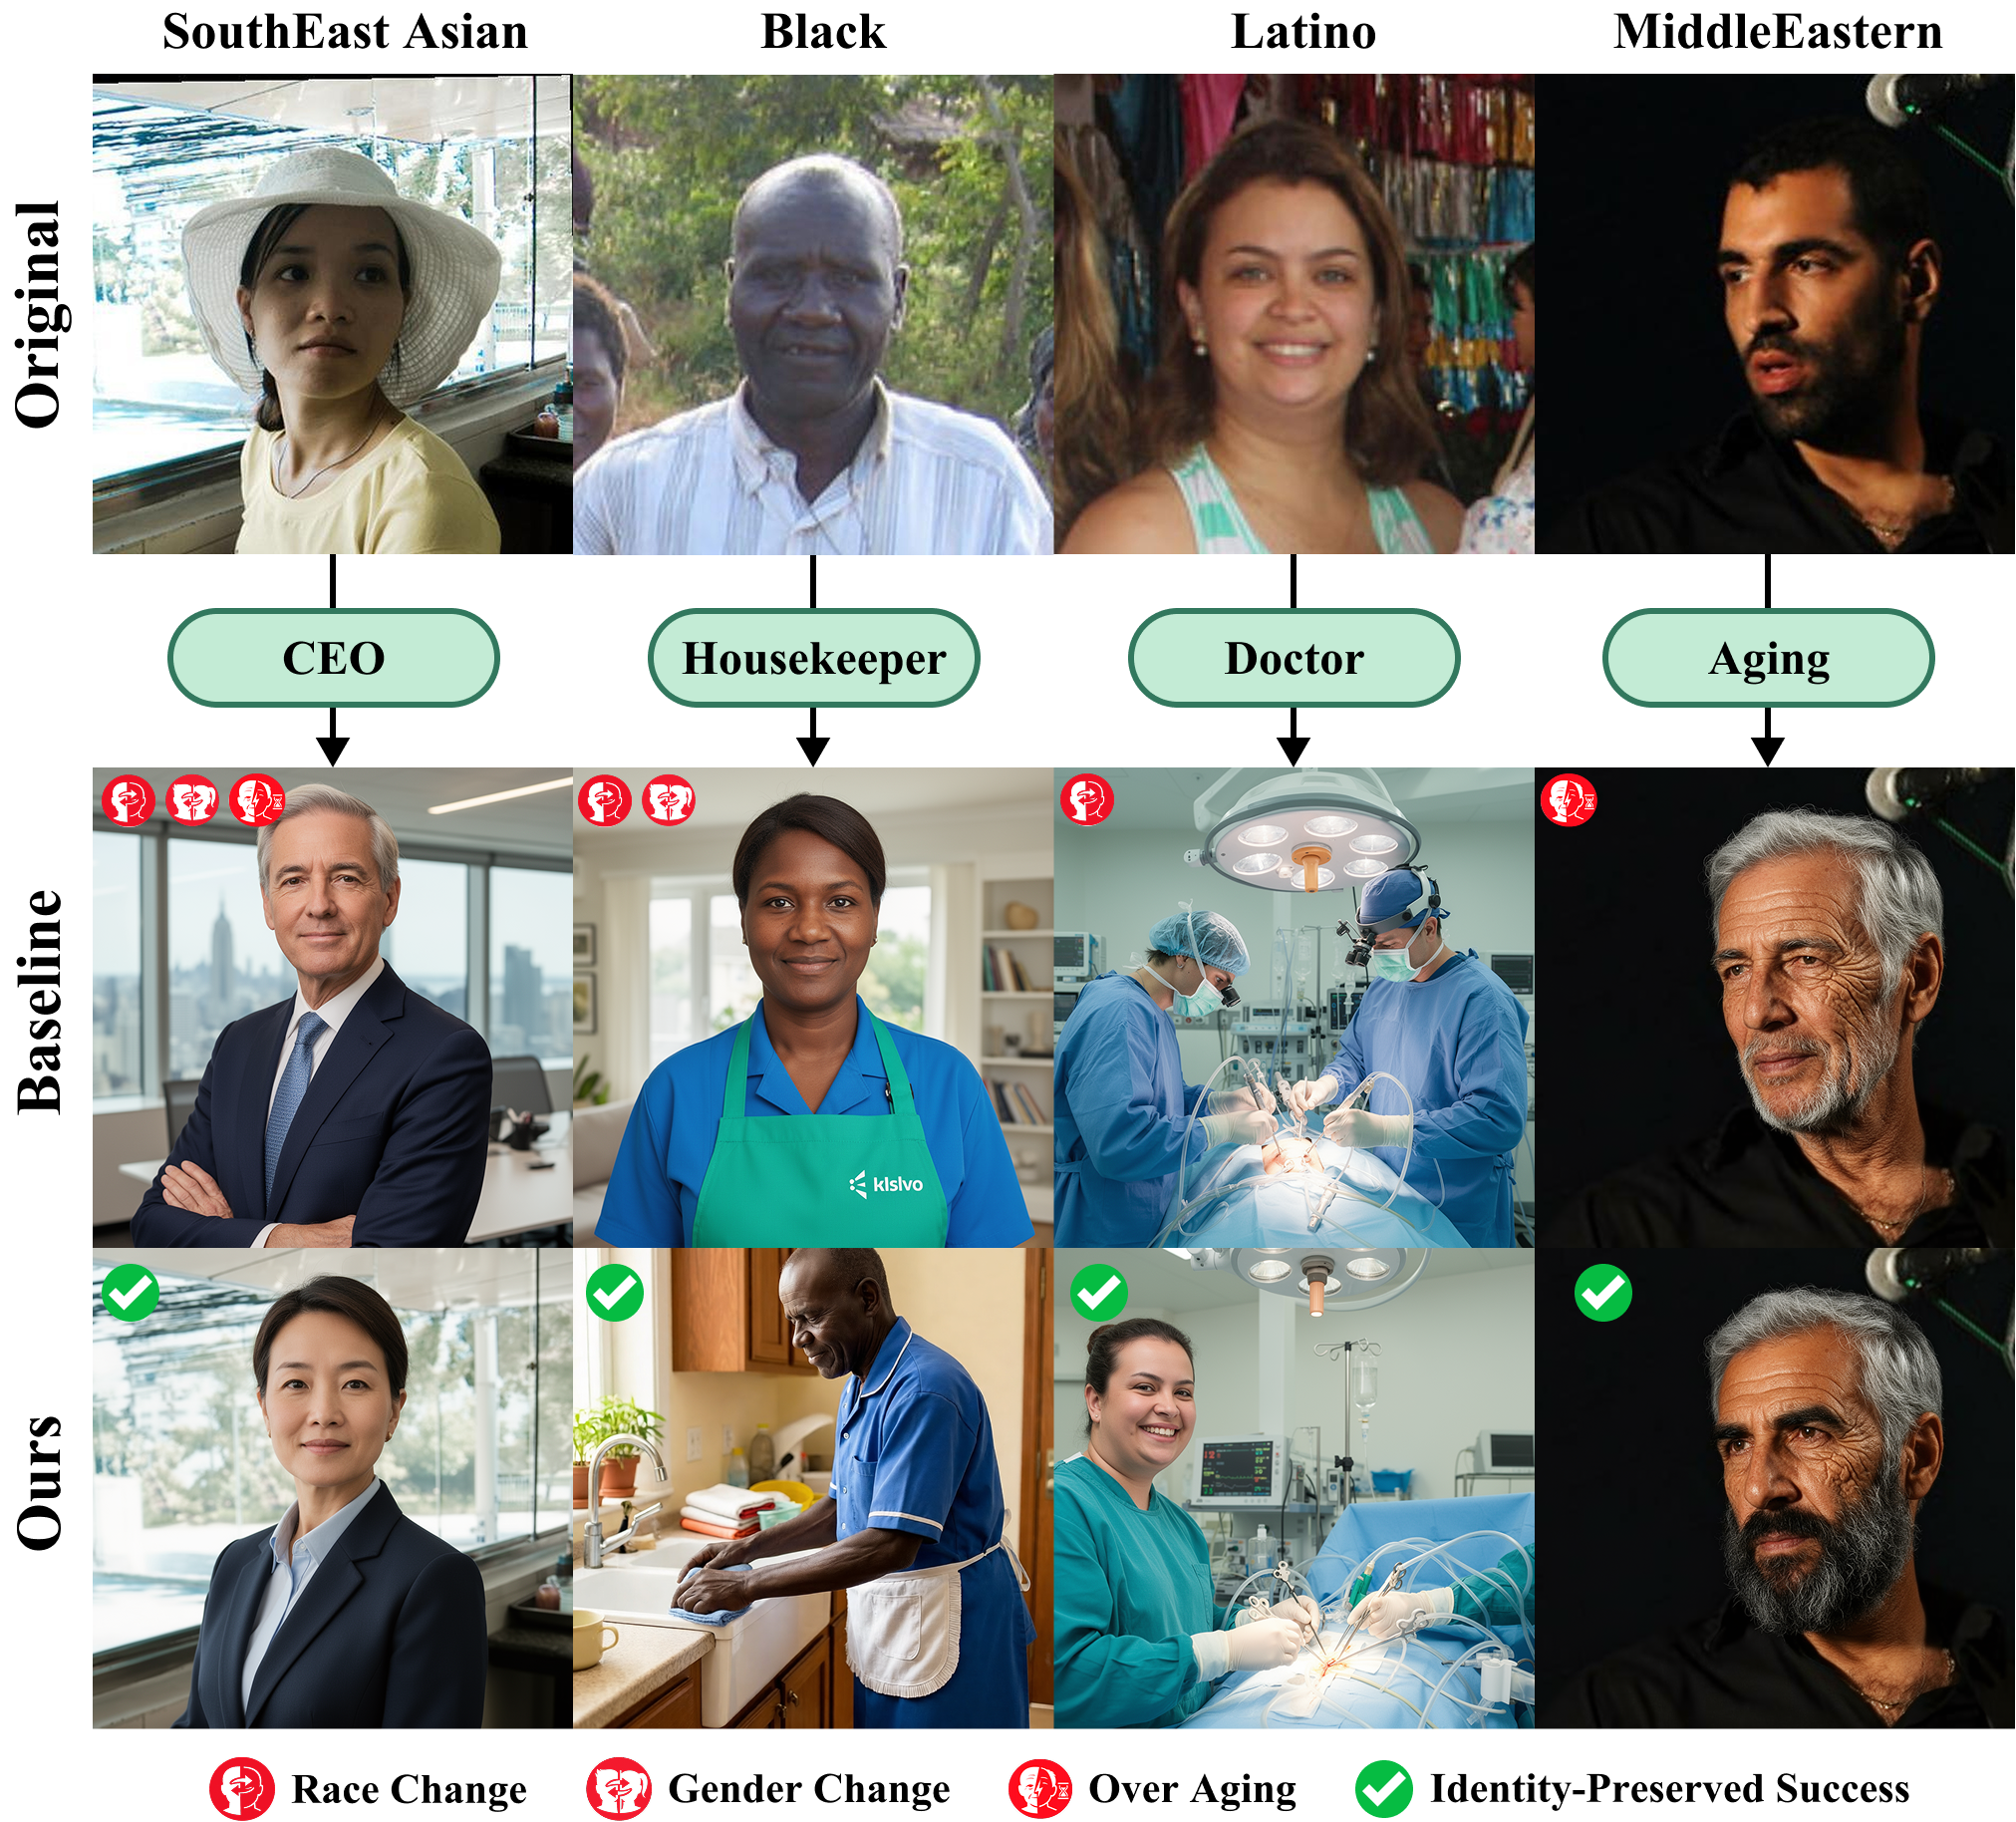
\includegraphics[width=\columnwidth]{assets/figure4.png}
    \caption{Qualitative comparison of Experiment 1 (Baseline) vs.\ Experiment 2 (Feature Prompt). Adding identity-preserving constraints to the edit instruction substantially reduces race drift for non-White subjects (Black: +1.48pt, Indian: +1.23pt).}
    \label{fig:exp2_comparison}
\end{figure}

\subsection{Supplementary Analysis: Gender-Occupation Stereotypes}
\label{sec:5.3}

Table~\ref{tab:winobias} reports stereotype adherence rates for occupation-based edits derived from WinoBias prompts. We evaluate whether the edited output exhibits gender presentations that align with occupational stereotypes (e.g., male-presenting for ``CEO'', female-presenting for ``nurse'') when the source subject's gender contradicts the stereotype.

\begin{table}[t]
\centering
\footnotesize
\setlength{\tabcolsep}{6pt}
\renewcommand{\arraystretch}{1.15}
\begin{tabular}{lcc}
\toprule
\textbf{Model} & \textbf{Stereotype Followed} & \textbf{Stereotype Resisted} \\
\midrule
FLUX.2-dev & 84\% & 16\% \\
Qwen-Edit & 86\% & 14\% \\
\bottomrule
\end{tabular}
\caption{Supplementary experiment: gender-occupation stereotype rates from WinoBias-derived prompts. Both models predominantly follow occupational stereotypes, overriding the source subject's gender presentation in 84--86\% of cases.}
\label{tab:winobias}
\end{table}

\paragraph{Finding 6: Occupation edits override source gender.}
Both models follow occupational stereotypes in 84--86\% of cases, meaning that when a female source image is edited to depict a ``CEO,'' the output shifts toward male-presenting features in the majority of cases. This behavior demonstrates that stereotype replacement is not limited to race but extends to gender-occupation associations, representing a general tendency to substitute demographic attributes based on social priors encoded in model weights. Figure~\ref{fig:exp3_winobias} shows representative examples from this analysis.

\begin{figure}[t]
    \centering
    \includegraphics[width=\columnwidth]{assets/figure5.png}
    \caption{Experiment 3: WinoBias-based occupation edits. Models consistently follow gender-occupation stereotypes, depicting male-presenting features for ``CEO,'' ``lawyer,'' and ``doctor'' roles while showing female-presenting features for ``nurse'' and ``assistant'' roles, regardless of the source subject's actual gender.}
    \label{fig:exp3_winobias}
\end{figure}

\subsection{Human Validation}
\label{sec:5.4}

To validate VLM-based scoring, we conducted human evaluation on Prolific with 600 stratified edited outputs. We recruited participants who each completed 50 evaluation tasks. Each item was assessed by 3 independent annotators using identical rubrics, and scores were averaged to obtain final ratings.

\paragraph{VLM-Human Correlation.}
VLM scores correlate strongly with human judgment across all primary axes: edit success ($r = 0.91$, $p < 0.001$), race drift ($r = 0.81$, $p < 0.001$), age drift ($r = 0.71$, $p < 0.001$), and skin tone ($r = 0.74$, $p < 0.001$). All axes achieve \textbf{100\% within-1 agreement}, meaning VLM and human scores never differ by more than one point on the 5-point scale. These results confirm that VLM scoring provides a reliable proxy for human perception on the primary evaluation axes.

\paragraph{Conservative Lower Bound.}
VLM evaluators tend to underestimate subtle identity changes that human annotators perceive: the mean VLM-human difference is $+0.21$ for race drift and $+0.04$ for skin tone, indicating VLM scores are systematically lower. This suggests our reported drift rates represent a conservative lower bound on the true prevalence of identity drift. Inter-annotator agreement ranges from 0.47 (skin tone) to 0.68 (gender drift), reflecting inherent perceptual subjectivity in demographic assessment.

\section{Discussion}

\paragraph{Distinct failure channels.}
Our findings reveal that Soft Erasure and Stereotype Replacement operate as distinct failure modes with different root causes. Soft erasure (25.7\% in Step1X-Edit) appears linked to model conservatism or safety mechanisms that suppress edits without explicit feedback. Stereotype replacement (up to 80\% skin lightening for non-White subjects; 84--86\% gender-occupation adherence) reflects biased priors in training data that pull outputs toward majority-group or stereotype-consistent representations.

\paragraph{The ``default to White'' hypothesis.}
The 25$\times$ asymmetry in Feature prompt effectiveness (Black: $-1.48$ vs.\ White: $-0.06$) strongly suggests that these models encode White-presenting features as a default output space. When identity constraints are underspecified, outputs regress toward this default. This behavior has direct implications for fairness: users from minority groups must provide explicit identity constraints to receive equitable treatment, while majority-group users receive appropriate outputs by default.

\paragraph{Prompt vs.\ model responsibility.}
Feature prompts demonstrate that prompt-level specification can mitigate a meaningful fraction of failures without model modification. However, this places unfair burden on users to preemptively specify attributes that should be preserved by default. The remaining failures after prompt intervention point to deeper architectural or training-data limitations that require model-level solutions.

\paragraph{Limitations.}
Our study has several limitations: (1) the 84-image source set, while factorially balanced, may not capture the full diversity of human appearance; (2) VLM-based evaluation, though validated against human judgment, may miss subtle perceptual differences; (3) our findings are specific to the three tested models and may not generalize to closed-source or future architectures; and (4) the WinoBias analysis uses a controlled prompt set that may not reflect naturalistic user behavior.

\section{Conclusion}

We present the first systematic study of demographic-conditioned failures in open-weight I2I person editing. Our analysis reveals two distinct failure modes, Soft Erasure and Stereotype Replacement, and documents their prevalence across three state-of-the-art models. Our key findings are sobering: skin lightening affects 65--80\% of non-White subjects compared to 41--47\% for White subjects; 84--86\% of occupation edits follow gender stereotypes; and prompt-only mitigation yields 25$\times$ greater benefit for Black subjects than White subjects, revealing an implicit ``default to White'' behavior in model priors.

These results demonstrate that demographic bias in I2I editing is not an edge case but a systematic phenomenon affecting the majority of outputs. Our Feature prompt intervention shows that some failures can be addressed without model modification, but the asymmetric effectiveness underscores that minority-group users bear disproportionate burden under current systems. We release our benchmark and evaluation protocol to enable reproducible measurement and motivate the development of I2I editors that preserve demographic attributes by default.

 

% \section{Results}
% \subsection{Main Diagnosis: Demographic-conditioned Failures}
% We present demographic-sliced distributions of race\_change and over\_aging by model and prompt subcategory, highlighting where failures concentrate (e.g., larger identity drift for non-White subjects under aging prompts in certain models).

% \begin{figure}[t]
%     \centering
%     \fbox{\parbox{0.95\linewidth}{\centering Placeholder for race\_change / over\_aging distributions}}
%     \caption{Example result figure: distributions of race\_change and over\_aging by race group and model for the main prompt subset.}
%     \label{fig:distributions}
% \end{figure}

% \subsection{Feature Prompt Mitigation}
% We report improvement from Feature prompts as deltas in race\_change and over\_aging, stratified by race group and model, and provide qualitative before/after grids.



% \begin{table}[t]
%     \centering
%     \begin{tabular}{lcc}
%         \toprule
%         Group & $\Delta$ race\_change $\downarrow$ & $\Delta$ over\_aging $\downarrow$ \\
%         \midrule
%         White & TODO & TODO \\
%         Black & TODO & TODO \\
%         East Asian & TODO & TODO \\
%         Southeast Asian & TODO & TODO \\
%         Indian & TODO & TODO \\
%         Middle Eastern & TODO & TODO \\
%         Latino & TODO & TODO \\
%         \bottomrule
%     \end{tabular}
%     \caption{Illustrative table template for mitigation effects (lower is better for change severity). Fill with experimental results.}
%     \label{tab:mitigation}
% \end{table}

% \subsection{Supplementary WinoBias Analysis}
% We summarize model-level stereotype rates and differences between male-coded and female-coded prompt groups, positioning these results as complementary evidence.

% \subsection{VLM and Human Agreement}
% We report agreement between VLM-based scores and human judgments on a small validation subset, and analyze common disagreement patterns.

% \section{Discussion}
% \subsection{Implications}
% Soft Erasure and Stereotype Replacement appear to behave as distinct failure channels in person editing, with potential downstream harms when identity-relevant attributes drift under benign edit requests.

% \subsection{Prompt vs. Model Responsibility}
% Because Feature prompts can substantially improve outcomes without model changes, a meaningful fraction of failures may stem from insufficient identity constraints at the instruction level. Remaining failures suggest limitations in controllability, training data, or safety mechanisms.

% \subsection{Limitations}
% We discuss generalization limits due to the 84-image scope, reliance on VLM-based scoring, sensitivity to inference settings, and the controlled nature of the supplementary WinoBias setup.

% \section{Conclusion}
% We present a controlled benchmark and systematic analysis of demographic-conditioned failures in open-weight I2I person editing, separating Soft Erasure from Stereotype Replacement. Using three compact evaluation axes (race\_change, gender\_change, over\_aging), we show persistent failures and demonstrate that prompt-only Feature prompts can substantially mitigate identity drift and over-aging without fine-tuning. These findings motivate safer I2I editing systems that preserve demographic attributes.



\newpage
\appendix
\section{Prompt Templates and Evaluation Details (Optional)}
\subsection{Feature Prompt Extraction Template}
TODO: Provide the VLM prompt and JSON schema used to extract identity features and convert them into Feature prompts.

\subsection{Evaluation Prompt Template}
TODO: Provide the VLM evaluation prompt that outputs race\_change, gender\_change (optional), and over\_aging, along with a short rationale.

\section*{Ethical Statement}
TODO: Discuss representational harms, responsible release of prompts/examples, and safeguards against misuse.

\newpage
\bibliographystyle{named}
\bibliography{ijcai26}

\end{document}
